% ============================================================
% DIAGRAM: Seq2Seq Encoder-Decoder (2014)
% ============================================================
% Caption: Figure 5.1: Seq2Seq encoder-decoder architecture.
%          (Adapted from Sutskever et al., 2014, p. 3105)
% ============================================================

\documentclass[tikz,border=10pt]{standalone}
\usepackage{tikz}
\usepackage{amsmath}
\usepackage{amsfonts}

\usetikzlibrary{shapes,arrows,positioning,fit,calc,backgrounds}

\begin{document}

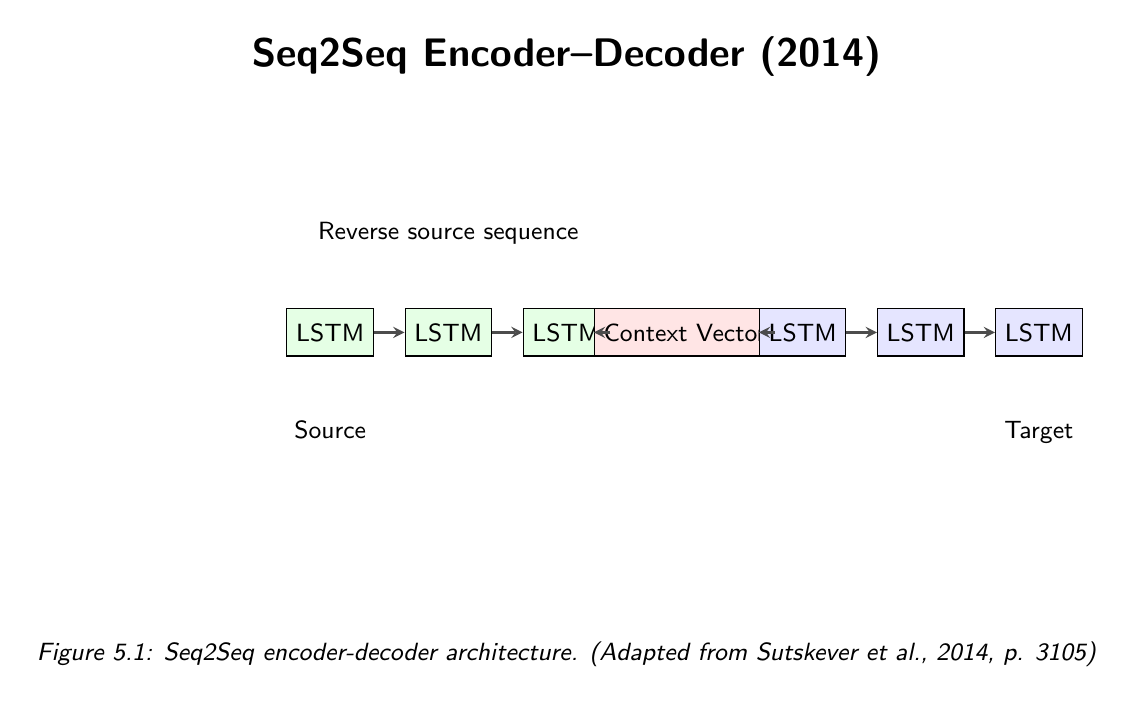
\begin{tikzpicture}[
    block/.style={draw, rectangle, minimum width=0.8cm, minimum height=0.6cm, fill=blue!10, font=\sffamily\small},
    edge/.style={-stealth, thick, draw=black!70},
    label/.style={font=\sffamily\small},
    title/.style={font=\sffamily\Large\bfseries},
    caption/.style={font=\sffamily\small\itshape},
]

\node[title] at (0, 3.5) {Seq2Seq Encoder–Decoder (2014)};

% Encoder
\node[block, fill=green!10] (enc1) at (-3, 0) {LSTM};
\node[block, fill=green!10] (enc2) at (-1.5, 0) {LSTM};
\node[block, fill=green!10] (enc3) at (0, 0) {LSTM};

% Context vector
\node[block, fill=red!10] (context) at (1.5, 0) {Context Vector};

% Decoder
\node[block, fill=blue!10] (dec1) at (3, 0) {LSTM};
\node[block, fill=blue!10] (dec2) at (4.5, 0) {LSTM};
\node[block, fill=blue!10] (dec3) at (6, 0) {LSTM};

% Input/Output labels
\node[below, font=\sffamily\small] at (-3, -1) {Source};
\node[below, font=\sffamily\small] at (6, -1) {Target};

\draw[edge] (enc1) -- (enc2);
\draw[edge] (enc2) -- (enc3);
\draw[edge] (enc3) -- (context);
\draw[edge] (context) -- (dec1);
\draw[edge] (dec1) -- (dec2);
\draw[edge] (dec2) -- (dec3);

% Reversal
\node[above, font=\sffamily\small] at (-1.5, 1) {Reverse source sequence};

\node[caption, anchor=north] at (0, -3.8) {
  Figure 5.1: Seq2Seq encoder-decoder architecture. (Adapted from Sutskever et al., 2014, p. 3105)
};

\end{tikzpicture}
\end{document}
